\documentclass{article}
\usepackage[utf8]{inputenc}
\usepackage{amsmath}
\usepackage{graphicx}
\usepackage{float}

\title{dADS 2 afl 2}
\author{Hanus Ejdesgaard Rindom 201303613\\
Christian Høj 201303530}
\date{April 2014}

\begin{document}

\maketitle

\section{Its party time}
We let $ c[x]= $ the conviviality of employee x, it is now the exercise to create a party list which has the highest combined conviviality:
$$ \text{MAX } \Sigma _{x \in S} c[x] $$
With the one rule that a parent/direct boss of an invited employee cannot be invited:
$$ \text{if } x \in S \text{ then } parent[x] \notin S $$

To solve this exercise we will use dynamic programming. To find the most optimal solution we will find the most optimal solution to the problem we will have to find the most optimal solution for the problems sub-problems.
we will describe the sub-problems as $ M(x) $ as the highest conviviality for the sub-problem where the employee x is included and use $ M^{'}(x) $  as the highest conviviality for the sub-problem where the employee x is not included\\
We can now use $ M(x) \text{ and } M^{'}(x) $ recursive:
$$ M(x) = c[x] + \Sigma _{y:parent[y] = x} M^{'}(y) $$
$$ M^{'}(x) = \Sigma _{y:parent[y] = x} \text{ max} { M(y),M^{'}(y) } $$

Where the first equation says that the optimal way to select employees, to the party, from x's sub-tree, is to select employees from the sub-tree y where y is not invited, x is included and the first (y) children is not.\\
The second equation says that the optimal way to select employees from x's sub-tree, is to select employees from the subtrees y of x, x is not invited and y is not necessarily invited.

We can now write a recursive code for the company tree in O(n) time:
\begin{figure}[H]
  \centering
    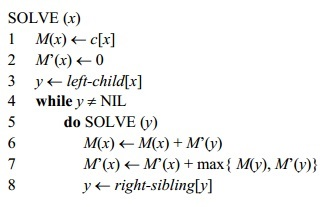
\includegraphics[width=0.50\textwidth]{Koala.jpg}
\end{figure}
This algorithm will begin when SOLVE(p) is called, where p is the president (The top of the tree). When the algorithm has ended will the highest sum of conviviality be given by $ \text{max } {M(p) \text{ , } M^{'}(p)} $\\
We have now found the highest sum of conviviality, we have yet to create a guest list, which can be done (again in O(n) time because we only go throug the list one time.):
\begin{figure}[H]
  \centering
    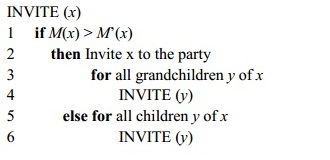
\includegraphics[width=0.50\textwidth]{hest.jpg}
\end{figure}
If $ M(p) > M^{'}(p) $ the optimal solution is to invite the big boss to the party\footnote{If realistic, he would have an insanely high conviviality, being the boss and all} and we can invite all the grandchildren to the party.\\
If it is the other way around $ M(p) < M^{'}(p) $ we can begin to look at the children of the president. Going through the tree recursively like this will leave us with a guest list with a conviviality sum matching the sum of the optimal solution $ \text{max } {M(p) \text{ , } M^{'}(p)} $.

\end{document}
